\documentclass[10pt,letterpaper,twocolumn]{article}
% \usepackage[twocolumn]{geometry}

% use Unicode characters - try changing the option if you run into troubles with special characters (e.g. umlauts)
\usepackage[utf8x]{inputenc}
% clean citations
\usepackage{cite}
% hyperref makes references clicky. use \url{www.example.com} or \href{www.example.com}{description} to add a clicky url
\usepackage{nameref,hyperref}
% line numbers
\usepackage[right]{lineno}
% improves typesetting in LaTeX
% \usepackage{microtype}
% degree symbol
\usepackage{gensymb}
\usepackage{amsmath}
\usepackage{booktabs}

% \DisableLigatures[f]{encoding = *, family = * }

% text layout - change as needed
% \raggedright{}
% \setlength{\parindent}{0.5cm}
% \textwidth 5.25in
% \textheight 8.75in

% Remove % for double line spacing
%\usepackage{setspace}
%\doublespacing

% use adjustwidth environment to exceed text width (see examples in text)
\usepackage{changepage}

% adjust caption style
\usepackage[aboveskip=1pt,labelfont=bf,labelsep=period,singlelinecheck=off]{caption}

% remove brackets from references
\makeatletter
\renewcommand{\@biblabel}[1]{\quad#1.}
\makeatother

% headrule, footrule and page numbers
\usepackage{lastpage,fancyhdr,graphicx}
\usepackage{epstopdf}
\pagestyle{myheadings}
\pagestyle{fancy}
\fancyhf{}
\rfoot{\thepage/\pageref{LastPage}}
\renewcommand{\footrule}{\hrule height 2pt \vspace{2mm}}
% \fancyheadoffset[L]{2.25in}
% \fancyfootoffset[L]{2.25in}

% use \textcolor{color}{text} for colored text (e.g. highlight to-do areas)
\usepackage{color}

% define custom colors (this one is for figure captions)
\definecolor{Gray}{gray}{.25}

% this is required to include graphics
\usepackage{graphicx}

% use if you want to put caption to the side of the figure - see example in text
\usepackage{sidecap}
\usepackage{hyperref}

% use for have text wrap around figures
\usepackage{wrapfig}
\usepackage[pscoord]{eso-pic}
\usepackage[fulladjust]{marginnote}
\reversemarginpar{}

% new commands
\newcommand{\cel}{\emph{C.~elegans}}
\newcommand{\fog}{\emph{fog-2}}
\newcommand{\ecol}{\emph{E.~coli}}

% gene numbers
\newcommand{\fogn}{1,881}
\newcommand{\agen}{5,592}
\newcommand{\interactionn}{1,318}
\newcommand{\coexpressed}{905}
\newcommand{\intersectn}{1,040}

% tf numbers
\newcommand{\tfaging}{145}
\newcommand{\tffog}{60}
\newcommand{\tfinteraction}{36}

% number of genes in gold standard
\newcommand{\goldn}{1056}
\newcommand{\goldfound}{506}
\newcommand{\goldpval}{$<10^{-38}$}

% website commands
\newcommand{\website}{\url{https://wormlabcaltech.github.io/Angeles_Leighton_2016/}}
\newcommand{\webref}{
\href{https://wormlabcaltech.github.io/Angeles_Leighton_2016/}{website}}

% more space between rows
\newcommand{\ra}[1]{\renewcommand{\arraystretch}{#1}}

\title{
  \Large
  \textbf{Transcriptomic Description of an Endogenous Female State in \cel{}}
}

\author{David Angeles-Albores\textsuperscript{1,$\dagger{}$}
\and{}
Daniel H.W. Leighton\textsuperscript{2,$\dagger{}$}
\and{}
Tiffany Tsou\textsuperscript{1}
\and{}
Tiffany H. Khaw\textsuperscript{1}
\and{}
Igor Antoshechkin\textsuperscript{3}
\and{}
Paul W. Sternberg\textsuperscript{1,*}
}

% document begins here
\begin{document}\sloppy{}
% \vspace*{0.35in}

% title goes here:
\twocolumn[
% title
\maketitle
% author info
\textbf{$\dagger$} These authors contributed equally to this work\\
\textbf{1} Department of Biology and Biological Engineering,
and Howard Hughes Medical Institute, Caltech, Pasadena, CA, 91125, USA\\
\textbf{2} Department of Human Genetics, Department of Biological Chemistry, and Howard Hughes Medical Institute, University of California, Los Angeles, Los Angeles, CA 90095, USA\\
\textbf{3} Department of Biology and Biological Engineering, Caltech, Pasadena, CA, 91125, USA\\
\textbf{*} Corresponding author. Contact:pws@caltech.edu
\section*{Abstract}
\bf{}  Understanding genome and gene function in a whole organism requires us to fully understand the life cycle and the physiology of the organism in question. Although it is traditionally though of as a hermaphrodite, \cel{} XX animals become (endogenous) females after 3 days of egg-laying. The molecular physiology of this state has not been studied as intensely as other parts of the life cycle, in spite of documented changes in behavior and metabolism that occur at this stage. To study the female state of \cel{}, we designed an experiment to measure the transcriptome of 1st day adult females, endogenous, 6th day adult females, as well as mutant feminized worms that never go through a hermaphrodite stage at these time points. Using this experimental design, we were able to measure the effects of biological aging from the transition into the female state.
We find that spermless young adult animals partially phenocopy 6 day old wild-type animals that have depleted their sperm after egg-laying, and that spermless animals also exhibit fewer transcriptomic changes associated with aging throughout these 6 days. Our results indicate that sperm loss is responsible for some of the naturally occuring transcriptomic changes that occur during the life cycle of these animals.
These changes involve a variety of factors, and they are enriched in transcription factors canonically associated with neuronal development and differentiation. Our data provide a high-quality picture of the changes that happen in global gene expression throughout the period of early aging in the worm.\vspace{10mm}
]
% now start line numbers
\nolinenumbers{}

% the * after section prevents numbering
\section*{Introduction}
\label{sec:introduction}

A challenge in understanding genome and gene function lies in obtaining a sense of the important components of organisms' life cycle and physiological states, e.g.\ stress. Here, we investigate what we argue is a distinct state in the \cel{} life cycle, the endogenous female state. \cel{} is best known as hermaphrodite, but after 3--4 days of egg-laying, the animals become sperm-depleted, which marks a transition into an endogenous female state. Transition into this state is marked by increased male-mating success~\cite{Garcia2001}, and an increased attractiveness to males~\cite{Morsci2011} at least partially through production of volatile chemical cues~\cite{Leighton2014}. Despite observations that the female state has differences in  behaviors and metabolism from the hermaphrodite, there is no description of this state. Here, we provide a general description of the transcriptomic changes that are apparent in female worms.


% % TODO middle paragraph
% While there has been a long-standing interest in \cel{} longevity and aging past 20 days of life, which has led to a rich literature~\cite{Kenyon1993,Antebi2007}, there has not been such intense study into the changes that occur during a period we refer to as `onset of aging'.
% We define onset of aging in \cel{} as the period of time that occurs between the first day of adulthood (post-L4 molt) and 6 days later, which is when viable oocytes shuts down~\cite{}. In this period of time, \cel{} worms also undergo a transition between a hermaphroditic, self-fertile stage and its final form as a true female worm that still has reproductive potential. Prior work has established that as hermaphroditic worms age and deplete their sperm, they become more attractive to males~\cite{Morsci2011}, and that this attraction is mediated at least partially by chemical cues~\cite{Leighton2014}. However, a transcriptional description of this transition has not been available before.

Since hermaphrodites are reproductive adults, the transition into the female state might also be accompanied by signs of aging. Simply comparing a hermaphrodite worm with an endogenous (post-hermaphroditic) female would not enable us to separate biological aging from post-reproductive development. We designed a two factor experiment to test our hypothesis. First, we examined wild type XX animals at the beginning of adulthood (before worms became visibly gravid) and after sperm depletion (6th day adults). Second, we examined feminized XX animals that always lack sperm but are fully fertile if supplied sperm by mating with males (see Fig.~\ref{fig:wormlife}).

\cel{} defective in sperm formation will never transition to a hermaphroditic stage. As time moves forward, these spermless worms should not exhibit changes related to sperm or fertility status, and should only exhibit onset of aging changes. Additionally, we reasoned that we might be able to identify gene expression changes due to different life histories: whereas hermaphrodites lay almost 300 eggs over three days, spermless females likely engage in more mate-seeking behavior. The different life histories could affect gene expression and aging.

As a model for a spermless female worm, we selected a \fog{} mutant for analysis. \fog{} is involved in germ-cell sex determination in the hermaphrodite worm and is required for spermatogenesis~\cite{Schedl1988,Clifford2000}. This protein is only expressed in the germline, which makes it a good target to generate spermless mutants with, since our perturbation would be targeted exclusively within the gonad.

Here, we show that during day 1 and day 6 of adulthood, we can detect a transcriptional signature associated with loss of hermaphroditic sperm and entrance into the endogenous female state; and we can also detect changes associated with onset of aging. First, loss of sperm leads to increases in the levels of transcription factors that are canonically associated with development and cellular differentiation, and enriched in neuronal functions.
Onset of aging also causes transcriptomic changes consisting of \agen{} genes in \cel{} and these changes are invariant between worms that undergo a hermaphroditic stage and worms that are always true females. To facilitate exploration of the data, we have generated a website with interactive plots. This website is located at: \website{}.

% figure experiment design
\begin{figure}[htbp]
\renewcommand{\familydefault}{\sfdefault}\normalfont{}
\centering
\captionsetup{width=\linewidth}
\includegraphics[width=\linewidth]{../output/figs/final_figs/worm_life_fog2_vs_n2.pdf}
\caption{Experimental design to identify genes associated with life-history.
}%
\label{fig:wormlife}
\end{figure}


\section*{Materials and Methods}
\label{sec:materials_methods}

\subsection*{Strains}
\label{sub:Strains}
Strains were grown at 20\degree{}C on NGM plates containing \ecol{} OP50~\cite{Brenner1974}. We used the laboratory \cel{} strain N2 as our wild-type strain. We also used the N2 strain containing the \fog{}\emph{(q71)} allele for all experiments. This strain was obtained from the CGC as strain JK574.


\subsection*{RNA extraction}
\label{sb:rna_extraction}
Synchronized worms were grown to either young adulthood or the 6th day of adulthood prior to RNA extraction. Synchronization and aging were carried out according to protocols described previously~\cite{Leighton2014}. 1000--5000 worms from each replicate were rinsed into a microcentrifuge tube in S basal (5.85g/L NaCl, 1g/L $\mathrm{K}_2\mathrm{HPO}_4$, 6g/L $\mathrm{KH}_2\mathrm{PO}_4$), and then spun down at 14,000rpm for 30s. The supernatant was removed and 1mL of Trizol was added. Worms were lysed by vortexing for 30s at room temperature and then 20 minutes at 4\degree. The Trizol lysate was then spun down at 14,000rpm for 10~minutes at 4\degree{} to allow removal of insoluble materials. Thereafter the Ambion TRIzol protocol was followed to finish the RNA extraction (MAN0001271 Rev. Date: 13 Dec 2012).

\subsection*{RNA-seq}
\label{sb:rna_seq}

RNA integrity was assessed using RNA 6000 Pico Kit for Bioanalyzer (Agilent Technologies \#5067--1513) and mRNA was isolated using NEBNext Poly(A) mRNA Magnetic Isolation Module (NEB \#E7490). RNA-seq libraries were constructed using NEBNext Ultra RNA Library Prep Kit for Illumina (NEB \#E7530) following manufacturer’s instructions. Briefly, mRNA isolated from $\sim1\mu$g of total RNA was fragmented to the average size of 200 nt by incubating at 94 °C for 15 min in first strand buffer, cDNA was synthesized using random primers and ProtoScript II Reverse Transcriptase followed by second strand synthesis using NEB Second Strand Synthesis Enzyme Mix. Resulting DNA fragments were end-repaired, dA tailed and ligated to NEBNext hairpin adaptors (NEB \#E7335).
After ligation, adaptors were converted to the ‘Y’ shape by treating with USER enzyme and DNA fragments were size selected using Agencourt AMPure XP beads (Beckman Coulter \#A63880) to generate fragment sizes between 250 and 350 bp. Adaptor-ligated DNA was PCR amplified followed by AMPure XP bead clean up. Libraries were quantified with Qubit dsDNA HS Kit (ThermoFisher Scientific \#Q32854) and the size distribution was confirmed with High Sensitivity DNA Kit for Bioanalyzer (Agilent Technologies \#5067- 4626).
Libraries were sequenced on Illumina HiSeq2500 in single read mode with the read length of 50 nt following manufacturer's instructions. Base calls were performed with RTA 1.13.48.0 followed by conversion to FASTQ with bcl2fastq 1.8.4.


\subsection*{RNA interference}
\label{sb:rnai}
RNAi was performed as described in previous protocols~\cite{Kamath2001} using a commercially available RNAi library~\cite{Kamath2003}. RNAi bacterial strains were grown in LB plus 100$\mu$g/mL ampicillin overnight. Fresh RNAi cultures were then plated onto NGM agar plates containing 25$\mu$g/mL carbenicillin and 1mM IPTG\@. N2 or \fog{}\emph{(q71)} hermaphrodites grown on \ecol{} OP50 were bleached onto sterile plates, and starved L1s transferred to recently seeded RNAi plates.
All assays were performed on the offspring of these L1s. Worms grown on every strain were monitored for gross abnormalities, such as sterility, lethality and larval arrest. Control worms in all assays were fed with an anti-GFP RNAi strain. All RNAi worms were grown at 20\degree{} C. All RNAi hits were sequence verified.

\subsection*{Oocyte dropping assay}
\label{sb:oocyte_assay}
We performed a slightly modified oocyte dropping assay based on previously described protocols~\cite{White2012}. Feminized \fog{}\emph{(q71)} hermaphrodites were picked as virgin L4s the day before the assay to a fresh RNAi plate. The following day, the adult animals were placed on assay plates (NGM agar seeded with 15$\mu$L of \ecol{} OP50 four days earlier), twenty worms per assay, and allowed to incubate at room temperature. Laid oocytes were counted after two hours. Plates were then left at room temperature overnight to serve as lawn-leaving assays.

\subsection*{Lawn-leaving assay}
\label{sb:lawn_leaving}
Lawn-leaving assays were performed as described previously~\cite{Lipton2004}. Young adult N2 hermaphrodites were selected the day of the assay and placed on assay plates (same as the oocyte dropping plates), twenty worms per assay, and allowed to incubate at room temperature overnight. Assays for \fog{}\emph{(q71)} hermaphrodites were performed on the same worms as used in the oocyte dropping assays. The following morning, plates were scored for leaving, with any worm touching any part of the bacterial lawn with any part of its body deemed to be “on” the lawn, and all others deemed to be “off”.

\subsection*{Brood size counting}
\label{sb:brood_size}
Worms were selected for this assay as L4 hermaphrodites to ensure that all progeny could be counted. For each replicate of each assay, a single worm was placed on a fresh RNAi plate and incubated at 20\degree. Every 1--2 days, the test worm was moved to a fresh RNAi plate, until it stopped laying eggs. Progeny were counted on each plate before they reached adulthood to ensure that only a single generation was counted.

\subsection*{Statistical Analysis}
\label{sb:statistics}
\subsubsection*{RNA-Seq Analysis.}
RNA-seq alignment was performed using Kallisto~\cite{Bray2015} with 200 bootstraps. The commands used for read-alignment are in the S.I.. Differential expression analysis was performed using Sleuth~\cite{Pimentel2016}. The following General Linear Model (GLM) was fit:

\begin{align*}
  \log(y_i) &= \beta_{0,i} + \beta_{G,i}\dot~G + \\
  &\beta_{A,i}\dot~A + \beta_{A::G,i}\dot~A~G,
  \label{eqn:GLM}
\end{align*}

where $y_i$ are the TPM counts for the ith gene; $\beta_{0,i}$ is the intercept for the ith gene, and $\beta_{X,i}$ is the regression coefficient for variable $X$ for the $i$th gene; $A$ is a binary age variable indicating 1st day adult (0) or 6th day adult (1) and $G$ is the genotype variable indicating wild-type (0) or \fog{} (1); $\beta_{A::G, i}$ refers to the regression coefficient accounting for the interaction between the age and genotype variables in the $i$th gene. Genes were called significant if the FDR-adjusted q-value for any regression coefficient was less than 0.1. Our script for differential analysis is available on GitHub.

Regression coefficients and TPM counts were processed using Python 3.5 in a Jupyter Notebook~\cite{Perez2007}. Data analysis was performed using the Pandas, NumPy and SciPy libraries~\cite{McKinney2011,VanDerWalt2011,Oliphant2007}. Graphics were created using the Matplotlib and Seaborn libraries~\cite{Waskom,Hunter2007}. Interactive graphics were generated using Bokeh~\cite{Team2014}.

Tissue Enrichment Analysis was performed using WormBase's TEA tool~\cite{Angeles-Albores2016} for Python.

\subsubsection*{Brood Size Analysis.}

Brood size results were analyzed using Welch's t-test to identify genes that were significantly different from a GFP RNAi control. RNAi control results were pooled over multiple days because we could not detect systematic day-day variation. We did not apply FDR or Bonferroni correction because, at a p-value threshold for significance of 0.05, we expected 1 false positive on average per screen.

\subsubsection*{Lawn-leaving Analysis.}

Lawn-leaving results were analyzed using a $\chi^2$ test for categorical variables. Results were considered statistically significant if $p<0.05$. No FDR or Bonferroni correction was applied because the size of the screen was too small, with 1 false positive expected on average per screen. However, the lawn-leaving results suffered from high variance, which can lead to false positive results.
To safeguard against false positive discovery, we used a non-parametric bootstrap to estimate the true $\chi^2$ value. Using a bootstrap on this dataset does not lead to statistical acceptance of any gene that was not accepted without a bootstrap; however, applying a boostrap does lead to statistical rejection of a large number of results.
\subsubsection*{Oocyte Dropping Analysis.}

Oocyte dropping results were analyzed using a non-parametric bootstrapped Mann-Whitney U-test because the GFP control variance was very large relative to the variance of the RNAi treatments. Results were considered statistically significant if $p<0.05$.


\subsection*{Data Availability}
\label{sb:data_availability}
Strains are available from the \emph{Caenorhabditis} Genetics Center upon request. All of the data and scripts pertinent for this project except the raw reads can be found on our github repository \url{https://github.com/WormLabCaltech/Angeles_Leighton_2016}. File S1 contains the Kallisto commands used to process the read alignments as well as the accession numbers for the raw-reads, whcih are available at GenBank. It also contains a detailed explanation for the format of files S2 and S3. File S2 contains the list of genes that were altered in aging regardless of genotype. File S3 contains the list of genes and their associations with the \fog{} phenotype. File S4 contains the genes that changed differently in aging wild-type worms and in \fog{} mutants. Raw reads will be deposited in the Sequence Read Archive and made available shortly.

\section*{Results}
\label{sec:results}
% figure (aging transcriptomics)
\begin{figure}[htbp]
\renewcommand{\familydefault}{\sfdefault}\normalfont{}
\centering
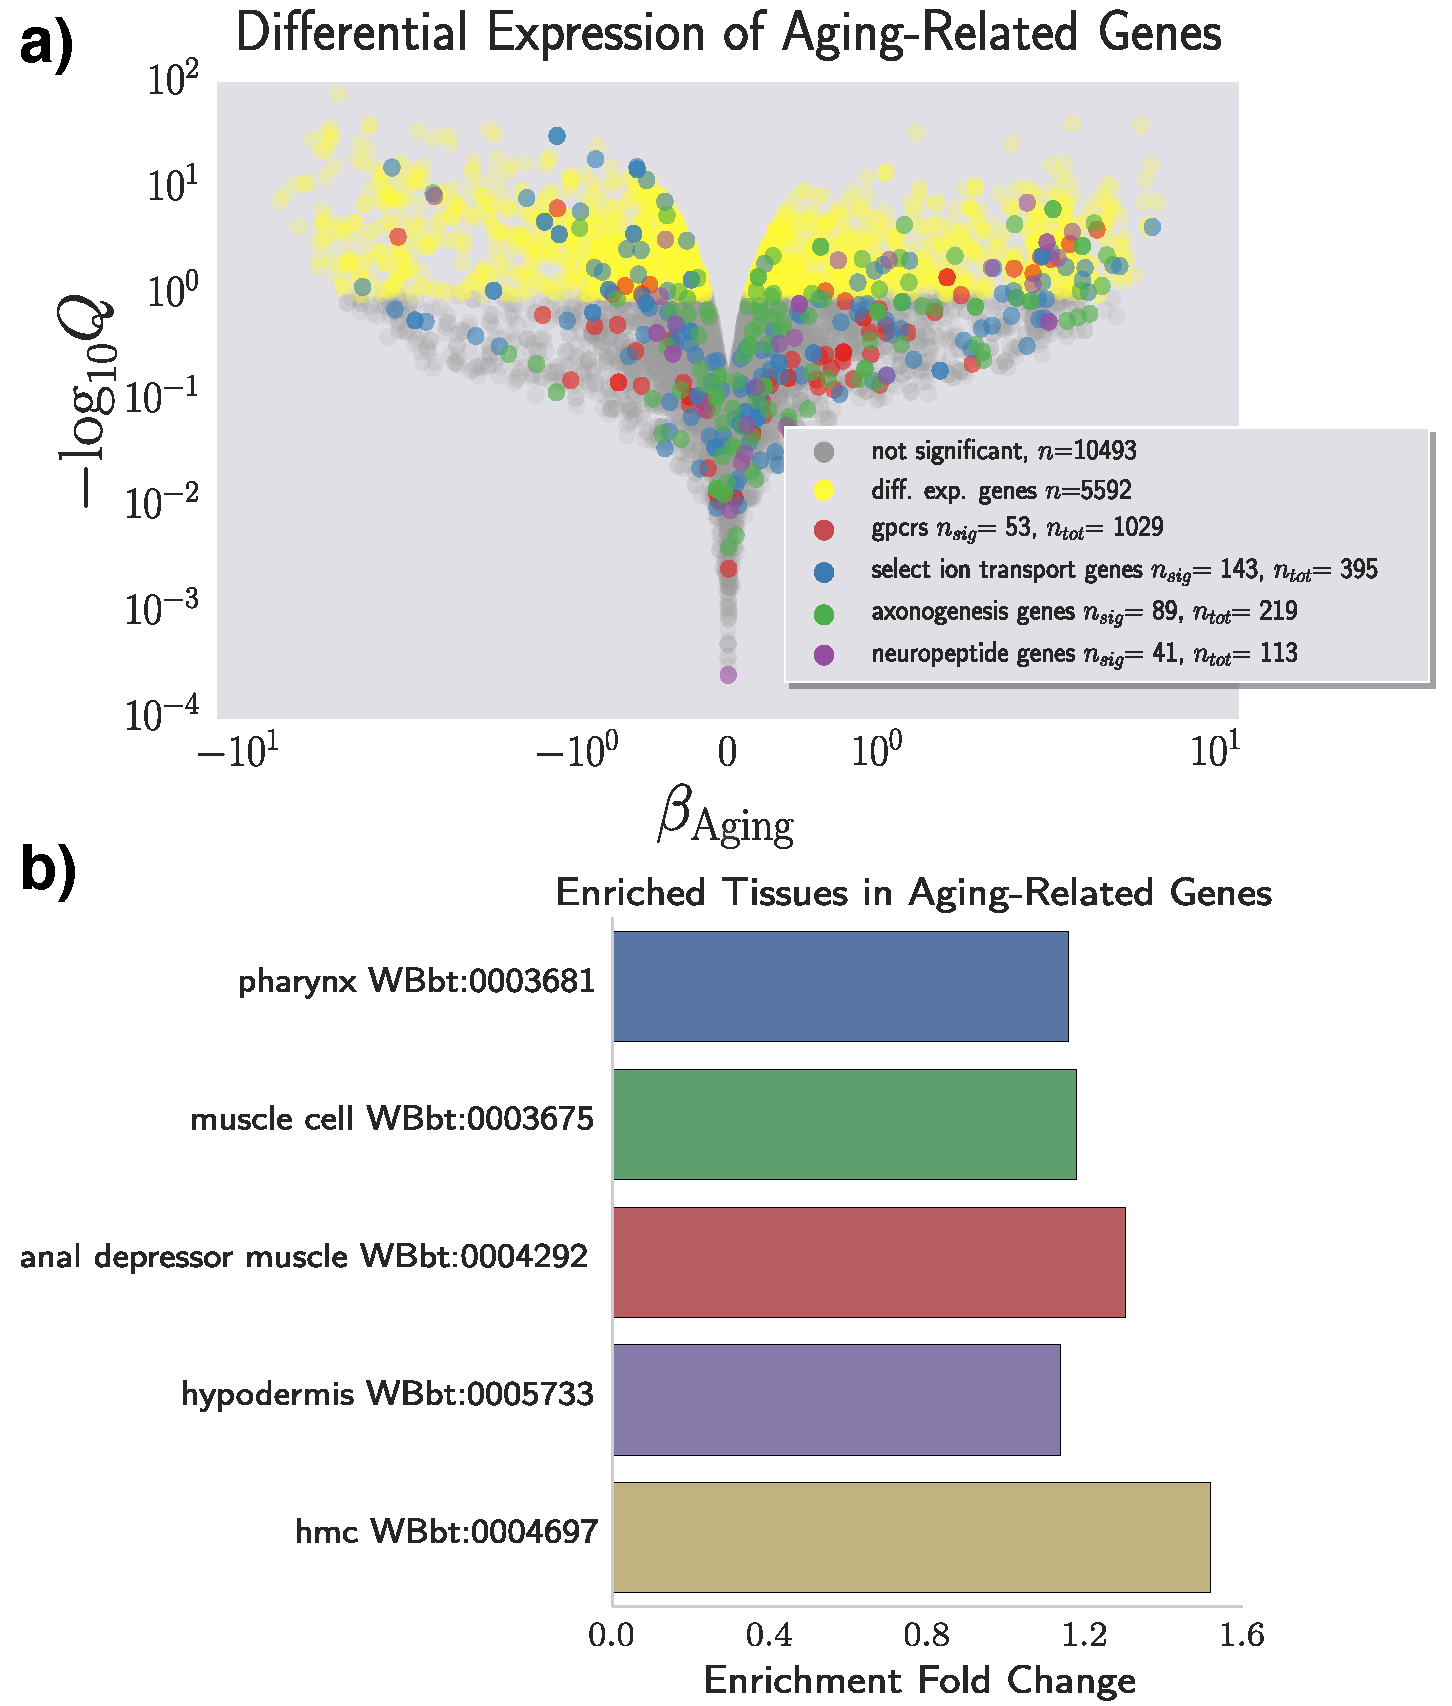
\includegraphics[width=\linewidth]{../output/figs/final_figs/aging_transcriptomics.pdf}
\caption{\textbf{ a} We identified a common aging transcriptome between N2 and \fog{} animals, which showed \agen{}  altered genes. The volcano plot was randomly down-sampled 30\%. Each point represents an individual isoform. \textbf{b} Tissue Enrichment Analysis showed that genes associated with muscle tissues and hypodermis are enriched in this dataset. Only statistically significantly enriched tissues are shown. An interactive version of this graph can be found on our \webref{}.
}
\label{fig:agingtranscriptome}
\end{figure}

\subsection*{Transcriptomics}
\label{sub:Transcriptomics}

We obtained RNA from 1st day adult animals before they were visibly gravid; post-hermaphroditic animals that were in the sixth day of adulthood; as well as from \fog{}\emph{(q71)} animals at these same timepoints. We obtained 16--19 million reads mappable to the \cel{} genome, which enabled us to identify 14702 individual genes totalling 21,143 isoforms.

We used a linear generalized model (see \nameref{sb:statistics}) with interactions to identify a transcriptomic profile associated with the \fog{} genotype, as well as a transcriptomic profile of \cel{} aging common to both genotypes. We identified an aging transcriptomic signature consisting of \agen{} genes that were differentially expressed in 6th day adult animals relative to 1st day adult animals. This constitutes almost one quarter of the genes in \cel{}. Tissue Enrichment Analysis (TEA) showed that muscle- and hypodermis-associated genes are particularly enriched in this dataset (see Figure~\ref{fig:agingtranscriptome}).

To verify the quality of our dataset, we generated a list of gold standard genes expected to be altered in 6th day adult worms using previous literature reports including downstream genes of \emph{daf-12}, \emph{daf-16}, and aging and lifespan extension datasets~\cite{Murphy2003,Halaschek-wiener2005,Lund2002,McCormick2012,Eckley2013}. We found \goldfound{} genes of \goldn{} genes in our golden standard. This result was statistically significant with a p-value \goldpval{}.

\begin{table*}
\renewcommand{\familydefault}{\sfdefault}\normalfont{}
\centering{}
\ra{1.3}
\caption{\textbf{Transcription Factor TEA Results.} We ran TEA on the transcription factors associated with aging. Raw results showed a large list of terms associated with embryonic tissues that are neuronal precursors (AB lineage), so we trimmed the results by removing any terms that were expected to show up less than once in our list (if a term is expected to show up $10^{-3}$ times in a list, 1 occurrence is enough to show enrichment in this list, leading to many false positives). The best 5 results by Q-value are shown below.}
\begin{tabular}{@{}lccr@{}}
\toprule{}
Tissue & Expected & Observed & Q-value\\
\bottomrule{}\\
P11 & 1 & 9 & $<10^{-5}$\\
ventral nerve cord &	9 &	26 &	$<10^{-5}$\\
dorsal nerve cord &	5 &	19 & $<10^{-5}$\\
head muscle & 3	& 13 &	$<10^{-4}$\\
P7.p & 1 &	6	& $<10^{-2}$\\
\bottomrule{}
\end{tabular}
\label{tab:tea_tf_age}
\end{table*}

We found \tfaging{} transcription factors in the set of genes altered in aging. We expected these transcription factors to reflect the same tissue enrichment as the bulk dataset, but the results showed enrichment of hypodermal tissues and neuronal tissues, not muscle (see Table~\ref{tab:tea_tf_age}). Many of these transcription factors have been  associated with developmental processess, and it is unclear why they would change expression in adult animals. Interactive volcano plots for each gene-set can be found in our \webref{}.

We were also able to identify \fogn{} genes associated with the \fog{} genotype, including \tffog{} transcription factors. Gonad-related tissues were enriched in this gene set, consistent with the function of \fog{} as a sperm specification factor. As before, tissue enrichment analysis of these transcription factors reveals that they are involved in neural development. Of the \fogn{} genes that we identified in the \fog{} transcriptome, \intersectn{} genes were also identified in our aging set. Moreover, of these \intersectn{}  genes, \coexpressed{} genes changed in the same direction in age and genotype.

We were surprised at the large fraction of genes that overlapped between these two categories. We built our model to explicitly avoid overlap between variables. Our original expectation had been that certain genes would show a common aging phenotype regardless of genotype; that \fog{} would exhibit a specific set of changes; and that a small set of genes would age differently between genotypes. However, the large fraction of genes that exhibit shared changes between both variables suggests that almost all genes that are associated with sperm loss through mutation of \fog{} have an aberrant aging behavior.

This aberrant behavior can be most clearly observed by plotting the $\beta$ regression coefficients for each variable against each other. Doing so reveals a clear trend along the line $y=x$. However, our model is built to specifically disallow this. The only situation in which $\beta_\mathrm{aging} = \beta_\mathrm{genotype}$ is a valid statement in our model is when $\beta_\mathrm{aging::genotype} \neq 0$. Therefore, we also plotted $\beta_\mathrm{aging::genotype}$ against $\beta_\mathrm{aging}$. This revealed a strong inverse relationship: The interaction term cancels the aging (or genotype) term. An old, \fog{} worm would be represented as
$\beta_\mathrm{aging} +\beta_\mathrm{genotype} + \beta_\mathrm{aging::genotype} = \beta_\mathrm{genotype}$.
Therefore, genes that are associated with sperm loss through mutation of \fog{} do not change through early aging in these animals. However, in animals that are wild-type, these same genes will eventually change to the same levels as in the \fog{} mutants. In other words, \fog{} partially phenocopies the aging process in wild-type animals 3 days post-adulthood (see Fig.~\ref{fig:aberrant_aging}).

% aberrant aging
\begin{figure}
\renewcommand{\familydefault}{\sfdefault}\normalfont{}
\centering
\includegraphics[width=\linewidth]{../output/figs/final_figs/aberrant_aging.pdf}
\caption{ \fog{} partially phenocopies early aging in \cel{}. The $\beta$ in each axes is the regression coefficient from the GLM, and can be loosely interpreted as an estimator of the log-fold change.
Feminization by loss of \fog{} is associated with a transcriptomic phenotype involving \fogn{} genes. \intersectn{}/\fogn{} of these genes are also altered in wild-type worms as they progress from young adulthood to old adulthood, and \coexpressed{} change in the same direction. However, progression from young to old adulthood in a \fog{} background results in no change in the expression level of these genes. \textbf{a)} We identified genes that change similarly in feminization as in aging. Black line is the line $y=x$, not a line of best fit. \textbf{b)} Many of the genes in \textbf{a} do not further change with age in a \fog{} animal.
The black line is the line $y=-x$, and is not a line of best fit. Color is proportional to $-\log{Q}$.
An interactive version of these graphs can be found on our \webref{}.
}%
\label{fig:aberrant_aging}
\end{figure}


\subsection*{Screens}
\label{subs:Screens}

% figure 3 (brood assay)
\begin{figure}
\renewcommand{\familydefault}{\sfdefault}\normalfont{}
\centering
\includegraphics[width=\linewidth]{../output/figs/final_figs/rnai_brood_assay_results.pdf}
\caption{Brood size screen results. GFP control RNAi is shaded in green. Results that are statistically significantly different from GFP are shaded in dark grey. Dotted red line shows the mean of the pooled GFP controls. Points are colored by the date the assay was started on.
}%
\label{fig:broodassay}
\end{figure}

To test whether the genes we identified might have phenotypes as single gene perturbations, we performed a series of screens that would identify phenotypes that are associated with sperm loss, namely sterility, altered lawn-leaving or ovulation rate.
% Brood Size Screen
We performed a brood size screen, selecting as targets genes that were upregulated in N2 but downregulated in \fog{}, although we also included a gene that was visually determined to have a sterile phenotype (\emph{zip-3}, which goes down with age). In total, we identified seven genes whose knockdown altered brood size (see Figure~\ref{fig:broodassay}). As expected, most of these genes were associated with decreased brood size. Of the six genes that showed decreased brood size, one had previously been described as having a sterile or lethal phenotype (\emph{ard-1}~\cite{Simmer2003}). \emph{exc-5} had not been described to have a sterile phenotype before. The remaining four genes that caused a decreased brood size had not been previously described to have a phenotype. R09H10.5 and WO7G4.5 had mild effects on brood size; whereas \emph{zip-3}, and R07E4.1 had strong effects on fertility. \emph{ard-1}, R09H10.5 and WO7G4.5 are all expressed in the intestine.
Although we cannot rule out that these genes are essential in development, there is a strong functional connection between the intestine and the germline through yolk production\cite{DePina2011}, and we hypothesize that these genes participate in communication between these tissues in adult worms.
We also identified \emph{ape-1} as a gene associated with increases in brood size. Given the small effect size, we cannot rule out that this is a false positive, even though we have applied a very conservative methodology to our statistical analysis.

% figure 5 (oocyte dropping)
\begin{figure}
\renewcommand{\familydefault}{\sfdefault}\normalfont{}
\centering
\includegraphics[width=\linewidth]{../output/figs/final_figs/oocyte_rate_assay.pdf}
\caption{Ovulation Rate Assay. GFP control RNAi is shaded in green. Results that are statistically significantly different from GFP are shaded in dark grey. Dotted red line shows the mean of the pooled GFP controls. Points are colored proportionally to their y-coordinate
}%
\label{fig:oocytedropping}
\end{figure}

Some of the genes in our genotype dataset could also be associated with ovulation rate in \fog{}. We selected genes that showed upregulation in \fog{} animals and placed them on a lawn for two hours. We observed large variation in the ovulation rate for the control RNAi, and as a result no genes were associated with alterations in ovulation rate. However, the pooled variance across the screen was very similar to the control variance, suggesting that our failure to identify genes was not a result of poor conditions or experimental variance. Our screen identified a single hit: C23H4.4, a predicted carboxyl ester lipase with unknown function.

% figure 4 (lawn-leaving)
\begin{figure}[htbp]
\renewcommand{\familydefault}{\sfdefault}\normalfont{}
\centering
\includegraphics[width=\linewidth]{../output/figs/final_figs/lawn_leaving_rnai_assay.pdf}
\caption{lawn-leaving Screen Results. GFP control RNAi is shaded in green. Results that are statistically significantly different from GFP are shaded in dark grey. Dotted red line shows the mean of the pooled GFP controls. Points are colored proportionally to their y-coordinate. \textbf{a} N2 lawn-leaving assay. \textbf{b} \fog{} lawn-leaving assay. Inset shows the screen-wide average lawn-leaving rate of N2 and \fog{}, which shows that the screen-wide lawn-leaving rate of \fog{} worms is twice the rate of lawn-leaving of N2 worms, in agreement with previous literature~\cite{Lipton2004}.
}%
\label{fig:lawnleaving}
\end{figure}

We also performed lawn-leaving assays because previous research has reported differences in hermaphrodite wild-type worms and virgin \fog{} leaving rates, and these differences are believed to be associated with differences in the status of the reproductive system~\cite{Lipton2004}. We tested genes that increased in \fog{} animals in a \fog{} background, expecting that decreasing these genes should lead to a reversal of the lawn-leaving assay. Likewise, we tested genes that were decreased in \fog{} animals in an N2 background, expecting that knockdown of these genes would cause lawn-leaving.
We identified 9 genes that had an altered lawn-leaving profile in an N2 background, and 9 genes that altered lawn-leaving profile in a \fog{} background. Oddly, both screens identified  genes that mainly stimulate lawn-leaving. Initially, we had expected that RNAi knockdown would allow us to identify genes that inhibit lawn-leaving behavior in an N2 background; whereas RNAi knockdown in a \fog{} background would identify genes that promote lawn-leaving. However, our screen only identified genes that suppress lawn-leaving in an N2 background. All other hits stimulated lawn-leaving.

% lawn leaving
% n2
% ZK131.11 - pathogen defense
% F42A10.7 - stress
% F17E9.3 - nan
% M01A8.1 - fat content
% C08F11.7 - nan
% exc-5 - lethal, dev variant, locomotion variant
% H24K24.4 - tRNA methyltransferase
% C14C10.2 - locomotion
% F59H6.5 - dna helicase, dauer

% fog2
% T10E9.3 - nan
% Y42G9A.2 - nan
% col-86 -cuticle
% unc-15 - egl
% nhx-6 - ion channel
% C23G10.6 - enzyme
% nhr-74 - tf
% F57F4.2 - nan
% R13A5.11 - involved in reproduction

\section*{Discussion}
\label{sec:discussion}

\subsection*{Defining an Early Aging Phenotype}
\label{sub:Defining an Early Aging Phenotype}

Our experimental design enables us to decouple the effects of egg-laying from aging. As a result of this, we identified a set of almost 4,000 genes that are altered similarly between wild-type and \fog{} mutants. Due to the read depth of our transcriptomic data (20 million reads) and the number of samples measured (3 biological replicates for 4 different life stages/genotypes), Constitutes the highest-quality description of the genetic changes that occur in any aging population of \cel{} yet published.
Although our data only capture $\sim50\%$ of the expression changes reported in earlier aging transcriptome literature, this disagreement can be explained by a difference in methodology; earlier publications typically addressed the aging of fertile wild-type hermaphrodites only indirectly.


\subsection*{Measurement of a female state}
\label{sub:female_state}

We set out to study the self-fertilizing (hermaphroditic) to self-sterile (female) transition by observing a worm that did not undergo this transition. In so doing, we were able to uncouple reproductive changes from the aging processes that sterile and fertile animals experience in common. A key prediction that emerges naturally from postulating the female state is that loss of the hermaphroditic stage should not impact the female-specific transcriptome. Moreover, as long as a female worm remains in this state, the transcriptome should reflect this permanence. Therefore, female worms should carry a transcriptomic signature, regardless of when the female transition ocurred (after an L4 stage or a hermaphroditic stage) and regardless of the worm's age.
Indeed, our results indicate the existence of a discrete female state. Genes associated with the female stage were largely invariant through time, as expected. Wild-type worms that aged into a female state exhibited the same changes. In a sense, the wild-type worms caught up to their \fog{} counterparts.


% We set out to prove the existence of a hermaphrodite-female transition by studying a worm that did not undergo this transition. In so doing, we were able to uncouple the effects of biological aging that adult worms undergo. A key prediction that emerges naturally from postulating the female state is that loss of the hermaphroditic stage should not impact the female-specific transcriptome. Moreover, as long as a female worm remains in this state, the transcriptome should reflect this permanence.
% Therefore, female worms that underwent a hermaphroditic stage should carry the transcriptomic signature associated with the female transition and worms that have always been female should have the same signature regardless of their age. Indeed, we measured such a state in the \fog{} genotype. Genes associated with the female stage were largely invariant through time, as expected. Wild-type worms that aged into a female state exhibited the same changes. In a sense, the wild-type worms caught up to their \fog{} counterparts.

\subsection*{Developmental Factors Change During Early Aging}
\label{sub:development_in_aging}

Our transcriptomes reveal a host of transcription factors that changed during early aging in \cel{}. Many of these transcription factors have been associated with development via cellular differentiation and specification. For example, we identified the transcription factor \emph{lin-32}, which has been associated with neuron development~\cite{Chalfie1989,Zhao1995,Portman2000}; the Six5 ortholog \emph{unc-39} has been associated with axonal pathfinding and neuron migration\cite{Yanowitz2004}; \emph{cnd-1}, a homolog  of the vertebrate NeuroD transcription factors, is expressed in the early embryo and is also involved in axon guidance~\cite{Schmitz2007}. Why these transcription factors turn on is a mystery, but we speculate that this hints at important neuronal changes that are taking place. Such changes might not be unexpected, given changes in behaviour and pheromone production that are known to occur as hermaphrodites age.

Our explorations shown that the loss of \fog{} phenocopies the endogenous female state in \cel{}.
Given the enrichment of neuronal transcription factors that are associated with sperm loss in our dataset, we believe this dataset should contain some of the transcriptomic modules that are involved in these pheromone production and behavioral pathways, although we have been unable to find these genes. Currently, we cannot judge how many of the changes induced by loss of hermaphroditic sperm are developmental (i.e., irreversible), and how many can be rescued by mating to a male.
While an entertaining thought experiment, establishing whether these transcriptomic changes can be rescued by males is a daunting experimental task, given that the timescales for physiologic changes could reasonably be the same as the timescale of onset of embryonic transcription. All in all, our research supports the idea that wide-ranging transcriptomic effects of aging in various tissues can be observed well before onset of mortality~\cite{Stroustrup2013}, and that the \cel{} continues to develop at this stage of its life as it enters a new part of its life cycle.

\section*{Acknowledgements}

We thank the \emph{Caenorhabditis} Genetics Center for sharing worm strains. This work would not be possible without the central repository of \cel{} information generated by WormBase, without which mining the genetic data would not have been possible. D.H.W.L. was supported by a National Institutes of Health US Public Health Service Training Grant (T32GM07616). This research was supported by the Howard Hughes Medical Institute, for which P.W.S. is an investigator.

\subsubsection*{Author Contributions:}
DA, DHWL and PWS designed all experiments. DHWL and THK collected RNA for library preparation. IA generated libraries and performed sequencing. DA performed all bioinformatics and statistical analyses. DA, TT and DHWL performed all screens. DA, DHWL and PWS wrote the paper.


\nolinenumbers{}

%This is where your bibliography is generated. Make sure that your .bib file is actually called library.bib
\bibliography{citations}

%This defines the bibliographies style. Search online for a list of available styles.
\bibliographystyle{plain}

\end{document}
